%= local definitions of macros ============================
\newcommand{\Herwig}{H\protect\scalebox{0.8}{ERWIG}\xspace}
\newcommand{\Pythia}{P\protect\scalebox{0.8}{YTHIA}\xspace}
\newcommand{\Sherpa}{S\protect\scalebox{0.8}{HERPA}\xspace}
\newcommand{\Rivet}{R\protect\scalebox{0.8}{IVET}\xspace}
\newcommand{\Recola}{R\protect\scalebox{0.8}{ECOLA}\xspace}
\newcommand{\Amegic}{A\protect\scalebox{0.8}{MEGIC}\xspace}
\newcommand{\Professor}{P\protect\scalebox{0.8}{ROFESSOR}\xspace}
\newcommand{\OpenLoops}{O\protect\scalebox{0.8}{PENLOOPS 2}\xspace}
\newcommand{\Collier}{C\protect\scalebox{0.8}{OLLIER}\xspace}
\newcommand{\Madgraph}{M\protect\scalebox{0.8}{G5\_aMC@NLO}\xspace}
\newcommand{\eps}{\varepsilon}
\newcommand{\mc}[1]{\mathcal{#1}}
\newcommand{\mr}[1]{\mathrm{#1}}
\newcommand{\mb}[1]{\mathbb{#1}}
\newcommand{\tm}[1]{\scalebox{0.95}{$#1$}}
\newcommand{\vp}{\ensuremath{\vphantom{\int_a^b}}}
\newcommand{\vP}{\ensuremath{\vphantom{\int\limits_a^b}}}

%= title + authors =====================================
\section{NLO corrections to off-shell \texorpdfstring{$WWW$}{WWW} production\protect\footnote{
  S.~Dittmaier,
  G.~Knippen,
  M.~Sch{\"o}nherr,
  C.~Schwan}{}}

%= MANDATORY label ======================================
\label{sec:WWW}

%= (optional) preamble ================================== 

%= intro ===== ==========================================
\subsection{Introduction}
\label{sec:WWW:intro}

ATLAS 8\,TeV analysis \cite{Aaboud:2016ftt}.


%= methods ===== ========================================
\subsection{Methods}
\label{sec:WWW:methods}

In this contribution, we are comparing the numerical results 
obtained by two different and independent calculations for 
off-shell $WWW$ production.
On the one hand side, we use a combination of \Sherpa 
\cite{Bothmann:2019yzt,Gleisberg:2008ta,Bothmann:2016nao,Hoeche:2014rya} 
and \Recola \cite{Actis:2012qn,Actis:2016mpe}, as presented 
in \cite{Schonherr:2018jva}. 
Therein, \Sherpa provides the tree-level matrix elements, 
infrared subtraction, process management and phase-space
integration through its matrix element generator \Amegic 
\cite{Krauss:2001iv,Gleisberg:2007md,Schonherr:2017qcj}. 
\Recola is interfaced \cite{Biedermann:2017yoi} to provide 
all renormalised virtual corrections.

On the other hand, the results denoted as DKS are the ones presented in Ref.~\cite{Dittmaier:2019twg}.
These numbers were calculated and double-checked using two private codes; the first one was developed specifically for this process, and the second one is a generic code that was already used to calculate other EW processes~\cite{Ballestrero:2018anz,Denner:2019tmn,Denner:2019zfp}.
The first code uses dipole subtraction as presented in Ref.~\cite{Catani:1996vz} for QCD corrections and Refs.~\cite{Dittmaier:1999mb,Dittmaier:2008md} for EW corrections.
Matrix elements were generated using \Madgraph \cite{Alwall:2014hca} and \Recola.
The second code is able to use either dipole subtraction as presented in Ref.~\cite{Catani:1996vz} for both QCD and EW corrections, the latter using the trivial substitutions for the Casimir operator presented e.g.\ in section 3.2 of Ref.~\cite{Kallweit:2014xda}, or, alternatively, the dipole subtraction methods used in the first code.
The matrix elements are provided by \OpenLoops \cite{Cascioli:2011va,Kallweit:2014xda,Buccioni:2019sur}, which uses \Collier \cite{Denner:2016kdg,Denner:2002ii,Denner:2005nn,Denner:2010tr} for the evaluation of rank 0 and 1 tensor one-loop integrals.
Both codes use multi-channel Monte Carlo techniques \cite{Hilgart:1992xu,Kleiss:1994qy} for the phase-space integration with phase-space maps similar to the ones presented in Ref.~\cite{Dittmaier:2002ap}.

All processes are calculated including all triple, double, 
single and non-resonant topologies, as well as all interferences 
between channels with different vector and Higgs boson intermediate
states.


%= comparison ===== =====================================
\subsection{Comparison and results}
\label{sec:WWW:comparison}

\begin{table}[t!]
  \centering
  \begin{tabular}{c|c}
    Cut & Value \\\hline
    $p_\mathrm{T}(\ell)$ & $[20,\infty]\,\text{GeV}$ \\
    $\eta(\ell)$ & $[-2.5,2.5]$ \\
    $p_\mathrm{T}(\ell_1)$ & $[27,\infty]\,\text{GeV}$ \\
    $\Delta R(\ell_i,\ell_j)$ & $[0.1,\infty]$
  \end{tabular}
  \caption{
    Definition of the fiducial region. Lepton requirements relate 
    to dressed leptons using a Cone algorithm with $\Delta R_\text{dress}=0.1$.
    \label{tab:WWW:cuts}
  }
\end{table}


\begin{table}[t!]
  \centering
  (i) $\mathrm{pp}\to e^-\mu^+\tau^+\bar{\nu}_e\nu_\mu\nu_\tau+X$\\
  \begin{tabular}{l|c|c|c|c|c}
    \hline
    13\,TeV \vP
    & LO [fb] & NLO [fb] 
    & $\delta_{q\bar{q}}^\text{EW}$ [\%]
    & $\delta_{q\gamma}^\text{EW}$ [\%]
    & $\delta^\text{QCD} [\%]$\\\hline
    \hfill DKS \vp
    & 0.194990(19) & 0.2626(10) & -7.70(40) & 7.220(5) & 38.02(04) \\
    \hfill\Sherpa{}+\Recola \vp
    & 0.195118(83) & 0.2649(21) & -7.38(57) & 7.217(3) & 38.11(10) \\\hline
  \end{tabular}\\[2mm]
  (ii) $\mathrm{pp}\to e^+\mu^-\tau^-\nu_e\bar{\nu}_\mu\bar{\nu}_\tau+X$\\
  \begin{tabular}{l|c|c|c|c|c}
    \hline
    13\,TeV \vP
    & LO [fb] & NLO [fb] 
    & $\delta_{q\bar{q}}^\text{EW}$ [\%]
    & $\delta_{q\gamma}^\text{EW}$ [\%]
    & $\delta^\text{QCD} [\%]$\\\hline
    \hfill DKS \vp
    & 0.118411(12) & 0.1597(06) & -7.00(30) & 7.260(5) & 37.17(4) \\
    \hfill\Sherpa{}+\Recola \vp
    & 0.118420(73) & 0.1584(14) & -6.73(51) & 7.267(3) & 37.07(9) \\\hline
  \end{tabular}
  \caption{
    Comparison of cross sections at 13\,TeV.
    \label{tab:WWW:xsecs13}
  }
\end{table}

\begin{table}[t!]
  \centering
  (i) $\mathrm{pp}\to e^-\mu^+\tau^+\bar{\nu}_e\nu_\mu\nu_\tau+X$\\
  \begin{tabular}{l|c|c|c|c|c}
    \hline
    14\,TeV \vP
    & LO [fb] & NLO [fb] 
    & $\delta_{q\bar{q}}^\text{EW}$ [\%]
    & $\delta_{q\gamma}^\text{EW}$ [\%]
    & $\delta^\text{QCD} [\%]$\\\hline
    \hfill DKS \vp
    & 0.209820(20) & 0.2872(12) & -7.80(40) & 7.780(5) & 40.04(04) \\
    \hfill\Sherpa{}+\Recola \vp
    & 0.209962(85) & 0.2898(23) & -7.47(59) & 7.793(4) & 40.10(11) \\\hline
  \end{tabular}\\[2mm]
  (ii) $\mathrm{pp}\to e^+\mu^-\tau^-\nu_e\bar{\nu}_\mu\bar{\nu}_\tau+X$\\
  \begin{tabular}{l|c|c|c|c|c}
    \hline
    14\,TeV \vP
    & LO [fb] & NLO [fb] 
    & $\delta_{q\bar{q}}^\text{EW}$ [\%]
    & $\delta_{q\gamma}^\text{EW}$ [\%]
    & $\delta^\text{QCD} [\%]$\\\hline
    \hfill DKS \vp
    & 0.129986(13) & 0.1779(07) & -7.20(40) & 7.730(5) & 39.15(04) \\
    \hfill\Sherpa{}+\Recola \vp
    & 0.130016(76) & 0.1766(15) & -6.81(55) & 7.738(4) & 39.18(10) \\\hline
  \end{tabular}
  \caption{
    Comparison of cross sections at 14\,TeV.
    \label{tab:WWW:xsecs14}
  }
\end{table}

To compare the independent
calculations laid out in the previous section we 
choose the following setup.
We compute the cross sections for the production of
final states with (at least) one electron, one muon, and one
$\tau$-lepton with the corresponding three neutrinos for the
LHC at 13 and 14\,TeV at leading and next-to-leading order
in both the QCD and electroweak coupling of the Standard Model
in the phase space detailed in 
Tab.~\ref{tab:WWW:cuts}.
The gauge boson masses and widths are defined by their on-shell 
value provided by the Particle Data Group \cite{Tanabashi:2018oca}, 
\begin{center}
  \begin{tabular}{ll}
    $M_W^\text{OS}=80.379\,\text{GeV}$\qquad & $\Gamma_W^\text{OS}=2.085\,\text{GeV}$ \\
    $M_Z^\text{OS}=91.1876\,\text{GeV}$\qquad & $\Gamma_Z^\text{OS}=2.4952\,\text{GeV}$.
  \end{tabular}
\end{center}
They are then converted to pole masses using 
\begin{equation}
  M_V=\frac{M_V^\text{OS}}{\sqrt{1+\left(\frac{\Gamma_V^\text{OS}}{M_V^\text{OS}}\right)^2}}\;,
  \qquad
  \Gamma_V=\frac{\Gamma_V^\text{OS}}{\sqrt{1+\left(\frac{\Gamma_V^\text{OS}}{M_V^\text{OS}}\right)^2}}.
\end{equation}
In addition, we set the Higgs boson and top-quark masses
and widths to 
\begin{center}
  \begin{tabular}{ll}
    $M_h=125\,\text{GeV}$ & $\Gamma_h=0.004088\,\text{GeV}$ \\
    $M_t=173\,\text{GeV}$ & $\Gamma_t=0$\;. \\
  \end{tabular}
\end{center}
All remaining quarks and leptons, in particular the bottom quark and the $\tau$-lepton,
are considered massless.
We perform our calculation in the complex mass scheme 
\cite{Denner:2005fg,Denner:2014zga},
defining
\begin{equation}
  \mu_V^2=M_V^2-\mathrm{i}M_V\Gamma_V\;.
\end{equation}
The CKM matrix is parametrised using the Cabibbo angle 
\begin{equation}
  \theta_\text{C}=0.22731\;,\nonumber
\end{equation}
neglecting mixing with the third generation. 
All parameters of the electroweak part of the Standard Model 
are fixed using the $G_\mu$-scheme \cite{Dittmaier:2001ay} with
\begin{equation}
  G_\mu=1.1663787\cdot 10^{-5}\,\text{GeV}^{-2}\;.\nonumber
\end{equation}
We then define the electromagnetic coupling through the 
real parts of the complex masses, i.e.\
\begin{equation}
  \alpha=\frac{\sqrt{2}}{\pi}\,G_\mu\,M_W^2\left(1-\frac{M_W^2}{M_Z^2}\right)\;.
\end{equation}
The electroweak parameters are renormalised in the same scheme.

The parton densities of the proton are parametrised using the 
NNPDF 3.1 QCD LO PDF set \cite{Ball:2017nwa} for the LO cross 
section, $\sigma^\text{LO}$, NNPDF 3.1 QCD+QED NLO PDF set 
\cite{Bertone:2017bme} for the Born contribution to the 
NLO calculation, $\sigma_1^\text{LO}$, and all genuine NLO 
corrections. 
We choose the PDF sets with the strong coupling set to
\begin{equation}
  \alpha_s(M_Z)=0.118\nonumber
\end{equation}
and \textsc{LHAPDF}\footnote{
  In particular, we use \textsc{LHAPDF} 6.2.1 with PDF sets 
  \texttt{NNPDF31\_lo\_as\_0118} and 
  \texttt{NNPDF31\_nlo\_as\_0118\_luxqed}.
} to evaluate them.
We set the renormalisation and factorisation scale to 
\begin{equation}
  \mu_\text{R/F}^2=\left(\vp3\,M_W\right)^2+\left(\sum\limits_{i\in S}\vec{p}_{\mathrm{T},i}\right)^2
\end{equation}
where $S$ denotes all colour-neutral final states.

We now define the relative NLO corrections 
\begin{equation}
  \delta_{q\bar{q}}^\text{EW}
  =\frac{\Delta\sigma_{q\bar{q}}^\text{NLO EW}}{\sigma_1^\text{LO}}
  \;,\qquad
  \delta_{q\gamma}^\text{EW}
  =\frac{\Delta\sigma_{q\gamma}^\text{NLO EW}}{\sigma^\text{LO}}
  \;,\qquad
  \delta^\text{QCD}
  =\frac{\sigma_1^\text{LO}-\sigma^\text{LO}+\Delta\sigma^\text{NLO QCD}}{\sigma^\text{LO}}\,,
\end{equation}
where the subscripts of the corrections $\Delta \sigma^\text{NLO}$
define the class of parton luminosities
that contribute.
Furthermore, $\sigma^\text{LO}$ denotes the LO integrated cross
section evaluated with LO PDFs, whereas $\sigma_1^\text{LO}$ denotes
the LO integrated cross section evaluated with NLO PDFs (as part of
the NLO prediction).
With these definitions, both the QCD correction and the photon
induced EW correction are defined w.r.t.\ the pure LO calculation,
while $\delta_{q\bar{q}}^\text{EW}$ is almost
entirely insensitive to the actual PDF chosen, and thus 
universal.


The results obtained with both calculations for this setup 
for both channels, $W^+W^+W^-$ and $W^+W^-W^-$, for the LHC 
at both 13 and 14\,TeV centre-of-mass energy are detailed 
in Tabs.\ \ref{tab:WWW:xsecs13} and \ref{tab:WWW:xsecs14}. 
We generally find good agreement, see Fig.~\ref{fig:WWW:xscomp},
despite the process's poor convergence owing to the presence
of multiple narrow resonances.

\begin{figure}[t!]
  \centering
  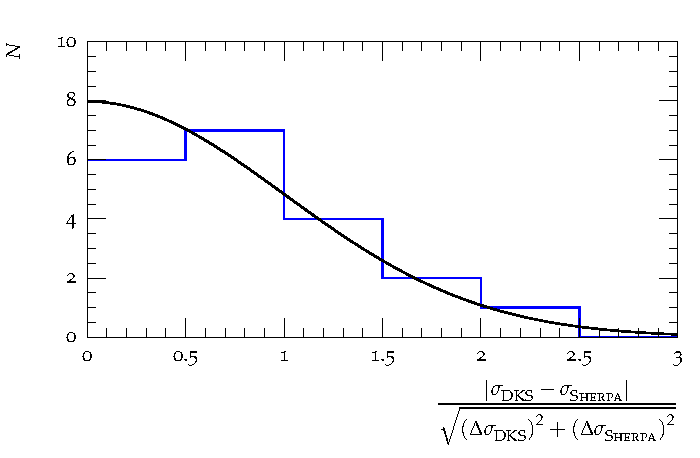
\includegraphics[width=0.5\textwidth]{comp-dist}
  \caption{
    Comparison of computed cross sections and relative 
    corrections of DKS and \Sherpa{}+\Recola. 
    For reference the black line 
    shows a properly normalised normal distribution.
    \label{fig:WWW:xscomp}
  }
\end{figure}





%= methods ===== ========================================
\subsection{Conclusions}
\label{sec:WWW:conclusions}



%= undefine macros (MANDATORY) ====================
\let\Herwig\undefined
\let\Pythia\undefined
\let\Sherpa\undefined
\let\Rivet\undefined
\let\Recola\undefined
\let\Professor\undefined
\let\Amegic\undefined
\let\OpenLoops\undefined
\let\Collier\undefined
\let\eps\undefined
\let\mc\undefined
\let\mr\undefined
\let\mb\undefined
\let\tm\undefined
\let\vp\undefined
\let\vP\undefined




